% !TEX root = ../../semexp-thesis.tex

\section{Semantic Conversations}
\label{sec:implementation/conversations}

To implement the exploratory programming agent in our prototype, we define several specializations of the \code{SemanticAgent} class from \semtex~(see \cref{sec:semtex/model/conversations}).
Each version of the agent contains instructions for a different type of semantic object interfaces as discussed in \cref{sec:design/agent/interfaces}: a conversation mode for object inspectors and a language extension for semantic messaging.

To add a new conversation mode to Squeak's inspector tools, we redirect all requests to the \code{Inspector} class by the toolset to a decorator.
This decorator inserts a new \code{chat} item into the inspector's field list, which references a conversation with our exploratory programming agent.
Second, the decorator embeds a minimal version of the conversation editor GUI of \semtex~(see \cref{sec:semtex/tools/editor}) for the agent when this field is selected~(\cref{fig:implementation/conversations/inspector}).

\begin{figure}
	\begin{minipage}{\textwidth}
		\centering
		% todo: reconsider relevance of screenshot and choice of example, update captions, move footnote into figure
		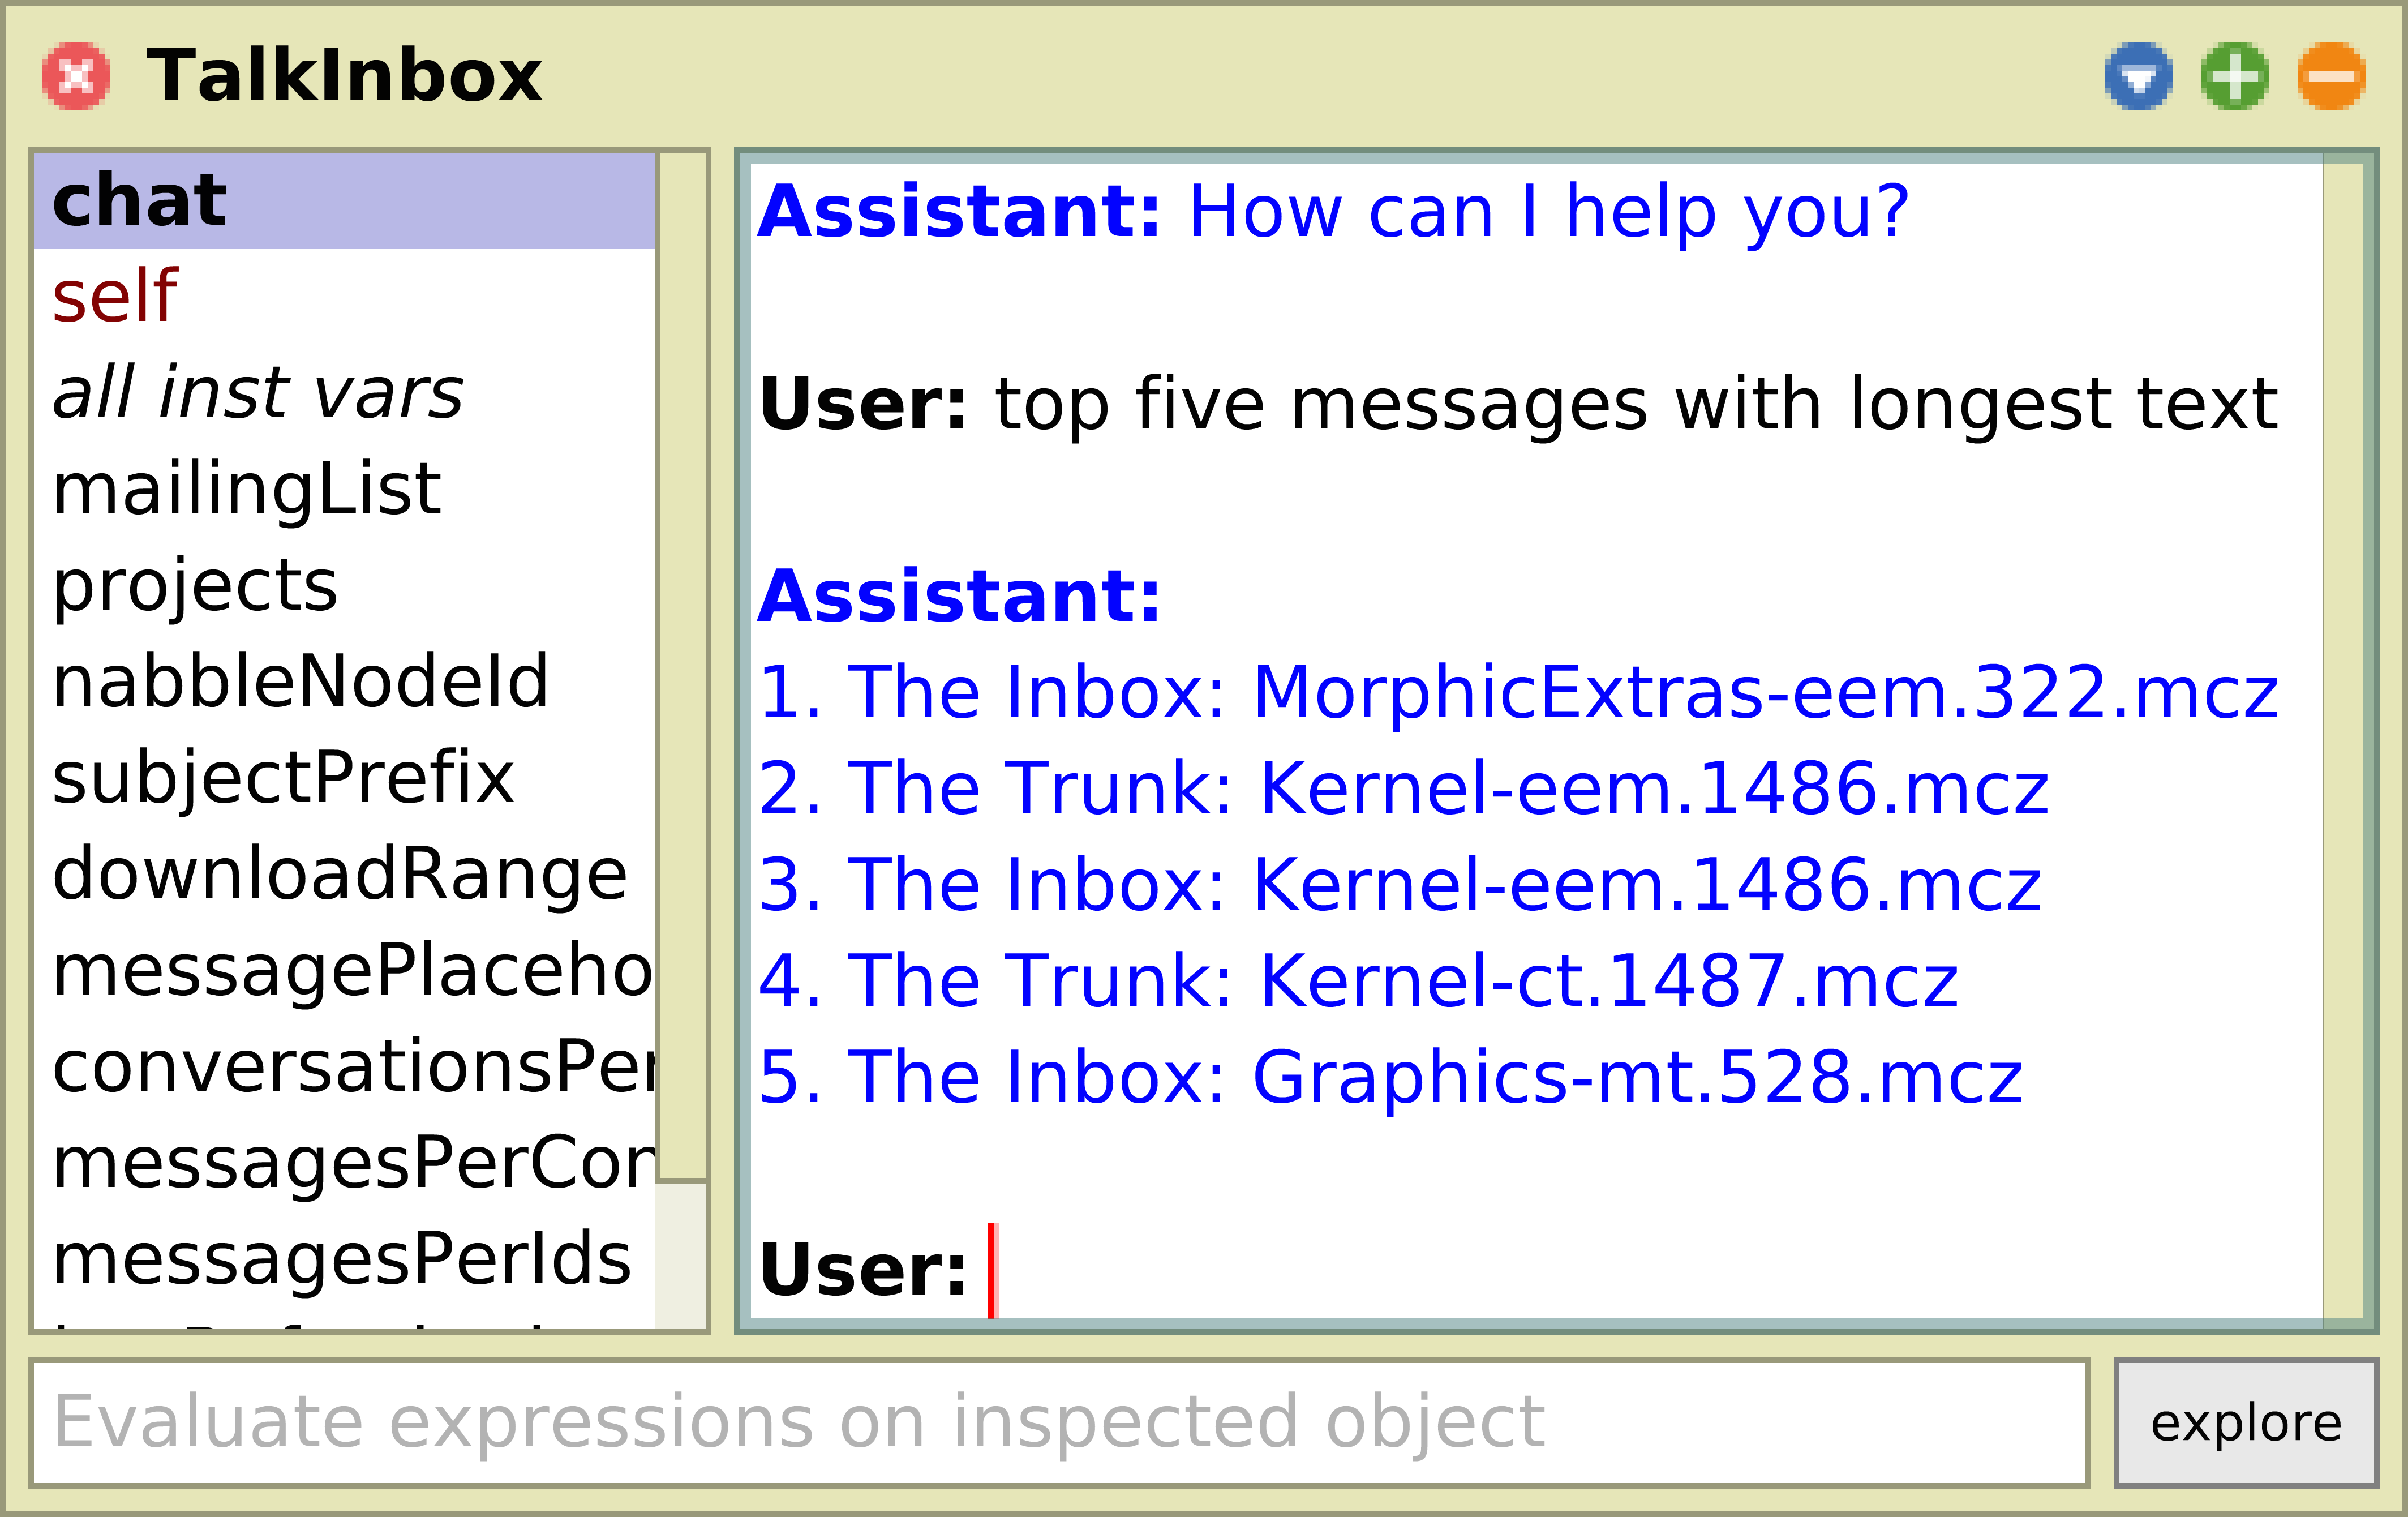
\includegraphics[width=.7\textwidth]{03_conversations/inspector.png}
		\caption[Our integration of a semantic conversational interface into Squeak's inspector.]{
			Our integration of a semantic conversational interface into Squeak's inspector (here: ``chat'' item in the field list on the left).
			In this example, the user chats with an archive of the Squeak mailing list\footnote{\url{https://github.com/hpi-swa-lab/squeak-inbox-talk}} to identify exceptionally large posts.
		}
		\label{fig:implementation/conversations/inspector}
	\end{minipage}
\end{figure}

To implement semantic messages in Squeak, we use the dynamic message-dispatch mechanism of Smalltalk's meta-object protocol by patching the method \code{Object>>\#doesNotUnderstand:}~\cite[sec.~5.11]{ingalls2020evolution} and forwarding all unknown messages to the agent.
Through an additional policy and a change in the function design (that is, by requiring an eventual call of the \code{evalAndReturn()} function from \cref{tab:agent/functions/interface}), we configure the agent to return Smalltalk objects instead of natural-language text.
Because we desired a distinction between regular and semantic messages during our experiments, we also implemented two alternative forms for expressing semantic messages:
\begin{description}[noextralabelsep]
	\item[Semantic proxies,] which are constructed explicitly and override \code{\#doesNotUnderstand:} to handle semantic messages:
	\begin{multicode}
		self semanticProxy mostOftenBoughtArticle.

		aProduct semanticProxy numberOfSalesTo: aCustomer.
	\end{multicode}
	\item[The \code{?} and \code{!} operators,] which take the semantic message as an argument selector:
	\begin{multicode}
		self ? \#mostOftenBoughtArticle.

		pendingOrders ! \#cancelItemsFromSpringSeries.
	\end{multicode}
	Here, the \code{?} operator indicates a declarative query for information.
	In contrast, the \code{!} operator permits side effects, allowing programmers to modify the state of objects in a semantic style.
\end{description}
While the \code{?} and \code{!} operators do not support additional arguments by design, we usually preferred them to semantic proxies in our experiments due to their reduced typing effort.
